\documentclass{article}
\usepackage{fullpage}
\usepackage{graphicx}
\usepackage{../svn-multi}
\svnid{$Id: simulator-user-manual.tex 87 2009-06-24 16:18:41Z jakebeal $}

\title{Proto Simulator User Manual}
\author{Jacob Beal}
\date{Date: \today, SVN Version: \svnrev{}}

\newcommand\todo[1]{\immediate\write16{TODO: #1}}
\newcommand\broken{{\em Not working!}}
\newcommand\experimental{{\em Experimental: behavior may be flawed and 
    may be changed without warning.}}

\newcommand\true{{\bf TRUE}}
\newcommand\false{{\bf FALSE}}

\newcommand\code[1]{\begin{quote}\var{#1}\end{quote}}

% arguments/keystrokes:
\newcommand\var[1]{{\tt #1}}
\newcommand\key[1]{{\bf #1}}
\newcommand\simarg[2]{\begin{quote} {\bf Argument: \var{#1}} \\ #2 \end{quote}}
\newcommand\simkey[2]{\begin{quote} {\bf Key: \key{#1}} \\ #2 \end{quote}}
\newcommand\simmouse[2]{\begin{quote} {\bf Mouse: \key{#1}} \\ #2 \end{quote}}
\newcommand\simargkey[3]{
  \begin{quote} {\bf Argument: \var{#1}, Key: \key{#2}} \\ #3 \end{quote}
}
\newcommand\simPMarg[3]{
  \begin{quote}
    {\bf Positive Argument: \var{#1}, Negative Argument: \var{#2}} \\ #3
  \end{quote}
}
\newcommand\simPMargkey[4]{
  \begin{quote}
    {\bf Positive Argument: \var{#1}, Negative Argument: \var{#2}, 
      Key: \key{#3}} \\ #4
  \end{quote}
}
% color
\newcommand\color[5]{{\bf (Color: {\tt #1} #2, #3, #4, #5)}} % name R G B A

\begin{document}

\maketitle

This is the user manual for the 2nd generation Proto simulator.  For
installation instructions, see the {\bf Proto Installation Guide}.  For
a reference of commonly used simulator and language commands, see the
{\bf Proto Quick Start}.  For a tutorial on the Proto language, see
the document {\bf Thinking In Proto}.  For a reference to the Proto
language, see the {\bf Proto Language Reference}.  For information on
how to extend the functionality of the simulator, see the {\bf Proto
Simulator Developer Reference}.

This manual is organized by functional modules within the simulator.
For each module, there is a brief description of the purpose and
behavior of the module, followed by a list of the command-line
arguments, keys, and colors used by that module.  Some modules
conflict in arguments and keys.  Ordinary keys are case sensitive
(i.e.  \key{c} and \key{C} are different); control keys are case
insensitive.

When arguments are described, an optional part of an argument is
surrounded by square brackets: \var{[]}.  Argument names always begin
with a dash.


% standard LaTeX credits insert; should echo AUTHORS

\section{Credits for Proto}

The Proto language was created in partnership by Jonathan Bachrach and
Jacob Beal.  As they created the language, Jonathan created the first
implementation of MIT Proto, including the first compiler, kernel,
simulator, and embedded device implementations.  Since that time, Jake
and other contributors have built on the work begun by Jonathan.

MIT Proto also includes contributions from (alphabetically):
%
Aaron Adler, Geoffrey Bays, Anna Derbakova, Nelson Elhage, Takeshi
Fujiwara, Tony Grue, Joshua Horowitz, Tom Hsu, Kanak Kshetri, Prakash
Manghwani, Dustin Mitchell, Omar Mysore, Maciej Pacula, Hayes Raffle,
Dany Qumsiyeh, Omari Stephens, Mark Tobenkin, Ray Tomlinson, Kyle
Usbeck, Dan Vickery

The Protobo platform code in platforms/protobo/ also includes 
Topobo-related code from (alphabetically):
%
  Mike Fleder, Limor Fried, Josh Lifton, Laura Yip



\section{Palette Files}

All colors used by the simulator are user-controllable: their default
values can be overridden with the use of palette files.

\simarg{-palette FILE}{Loads the palette in \var{FILE}.  This
command can be invoked multiple times, loading multiple palettes.
Palettes load in the order they are specified on the command line,
with later entries possibly overriding earlier ones.}

Palette files are formatted as follows:
\begin{itemize}
\item Whitespace is ignored
\item '\#' as first non-whitespace character in a line indicates a comment
\item One color per line, specified \var{NAME RED GREEN BLUE [ALPHA]},
      where \var{NAME} is the name of the color, and the others are
      values between zero and one.  If unspecified, \var{ALPHA} defaults
      to 1.0, which is solid.
\end{itemize}
Each specified color replaces only the current value assigned to that
color, so multiple palette files can be layered, each changing only a
portion of the colors.

\paragraph{Example Palette File:}
\begin{quote}
\begin{verbatim}
# Turn the background a horrid pink
BACKGROUND 1 0.8 0.8 1  
  # Make the devices green and the times translucent cyan and white
SIMPLE_BODY 0 1 0  
TIME_DISPLAY 0 1 1 0.5
FPS_DISPLAY 1 1 1 0.3
\end{verbatim}
\end{quote}


\section{Core Simulator}

The core functions of the simulator are to create a simulation,
control its progress, and manage the user interface.

If there is precisely one unhandled argument, that argument is taken
to be the Proto script to run.  If there are no unhandled
arguments, the script defaults to \var{(app)}.  If there are multiple
unhandled arguments, the simulator gives a warning and uses the last
one as the script.

\simarg{-seed N}{Use \var{N} as a random seed, defaults to a value set
  by the current time.}
\simkey{q}{Quit the simulator.}

\simarg{-mag N}{Relative magnification of text displays for each device,
  default 1.}
\simargkey{-i}{i}{Show the ID of each device \color{DEVICE\_ID}{1}{0}{0}{0.8}.
  Toggled by key.}

\paragraph{Starting, Stopping, and Running:}
\simargkey{-T}{T}{Display simulator time in lower left corner
  \color{TIME\_DISPLAY}{1}{0}{1}{1} and frames-per-second in lower
  right corner \color{FPS\_DISPLAY}{1}{0}{1}{1}. Toggled by key.}
\simargkey{-step}{s}{Use stepping mode, advancing one step on key \key{s}}
\simkey{x}{Execute freely (ending stepping mode).}
\simarg{-stop-after N}{Terminate after \var{N} simulated seconds,
  default infinity.}
\simargkey{-throttle}{X}{Throttle simulated time to advance relative
  to real time (toggled by key).  When the simulator cannot keep up, a
  warning appears in the lower center
  \color{LAG\_WARNING}{1}{0}{0}{1}}
\simarg{-ratio N}{Ratio between real time and simulated time when
  throttling is active, default 1}
\simarg{-s N}{Set simulated seconds per step, default 0.01/\var{ratio}}


\simkey{CTRL-s}{Slow throttled simulator.  Each keystroke
    divides speed by $2^{\frac{1}{4}}$}
\simkey{CTRL-a}{Accelerate throttled simulator.  Each keystroke
  multiplies speed by $2^{\frac{1}{4}}$}
\simkey{CTRL-d}{Return throttled simulator to a ratio of 1:1 simulated to real 
  time.}

\paragraph{Display:}
The display background is colored \color{BACKGROUND}{0}{0}{0}{0.5}.

\simarg{-window-name NAME}{Title the simulator window \var{NAME}, 
  default ``Proto Simulator''}
\simargkey{-f}{f}{Full screen display (toggled by key)}
\todo{Need to add GLUT geometry arguments}
\simarg{-headless}{Run without a display or user interface;
  default \false{} unless compiled without OpenGL.  When headless,
  \var{-stop-after} must be specified.}

\simkey{PAGE UP}{Zoom in.}
\simkey{PAGE DOWN}{Zoom out.}
\simkey{z}{Reset display to initial view.}
\simkey{ARROW KEYS}{Shift simulation display in the direction of the arrow, 
  in the simulation's coordinate system.}
\simmouse{LEFT DRAG}{Rotate display.}
\simmouse{RIGHT DRAG}{Zoom display; toward center zooms out, away zooms in.}
  
\paragraph{Selection:}
Selected devices are indicated with a thin ring
\color{DEVICE\_SELECTED}{0.5}{0.5}{0.5}{0.8} four times the device's
body diameter,

\simmouse{LEFT CLICK}{Select the devices clicked on.}
\simmouse{RIGHT CLICK}{Select, then print the state of the selected
  device(s) to standard out.}
\simmouse{SHIFT LEFT DRAG}{Toggle the selection of all devices in a
  rectangular display region.  The area to be selected is colored
  \color{DRAG\_SELECTION}{1}{1}{0}{0.5}.}
\simmouse{SHIFT RIGHT DRAG}{Move selected devices.}
\simkey{U}{Unselect all devices.}

\paragraph{Code}
\simkey{l}{Recompile and reload the current script, injecting at
  the selected devices.}
\simarg{--platform PLAT}{Use the platform \var{PLAT}.  This causes
  proto to look for the files
  \code{\var{\$datarootdir}/proto/platforms/\var{PLAT}/platform\_ops.h}
  and \var{platform\_ops.proto} to define the platform-specific ops
  that the compiler will use.}
\simarg{--path PATH}{Add the directories in \var{PATH} to the front of the list
  of directories searched when looking for files (e.g. Proto programs).  By
  default, the path contains \var{.} (the current directory) and
  \var{\$libdir/proto/}.}
\simarg{--basepath PATH}{Override the default Proto path, substituting
  \var{PATH} instead.}
\simarg{--print-ast}{During compilation, print out the intermediate
  abstract-syntax-tree form. \experimental{}}
\simarg{--instructions}{After compiling, print the script instructions
  that have been generated, in the form of a C array includable in a 
  header file. \experimental{}}
\simargkey{-k}{k}{Display the current script across the middle of the window
  (toggled by key). \broken{}}
\simargkey{-show-script-version}{j}{Show what version of the script is
  loaded at each device \color{DEVICE\_SCRIPT}{1}{0}{0}{0.8}.  Toggled
  by key.}
\simargkey{-v}{n}{Show value computed at each device 
  \color{DEVICE\_VALUE}{0.5}{0.5}{1}{0.8}.  Toggled by key.}
\simargkey{-sv}{v}{When device outputs a 2- or 3-tuple, display it as
  a vector (toggled by key).  The vector is interpreted as meters,
  drawn as a line \color{VECTOR\_BODY}{0}{0}{1}{0.8} with a
  differently colored tip to indicate direction
  \color{VECTOR\_TIP}{1}{0}{1}{0.8}.}
  

\section{Debugging}

The debugger logs chosen types of activity to standard out.  To
prevent complete overload, debugging information flows only when
global debug mode is on and then only from devices selected for
debugging.  In that case, debugging information from designated
categories prints to standard out from the devices selected for debugging.
Devices currently logging debugging information are shown by a filled
disc twice the size of the device
\color{DEVICE\_DEBUG}{1}{0.8}{0.8}{0.5}.

For example, to get a trace of networking activity in the kernel, add
the command line arguments \var{-g -debug-kernel}, then select the
desired devices and hit \key{D}.

\simkey{D}{Toggle selection for debugging on selected devices.}
\simargkey{-g}{d}{Global debug mode (toggled by key)}
\simargkey{-t}{a}{When debugging, post trace of evaluation in kernel
  of debug devices (toggled by key).}
\simarg{-debug-kernel}{When debugging, post trace of networking
  activity in kernel}
\simarg{-debug-script}{When debugging, post trace of viral code
  distribution in in kernel}


\section{State ``Dumping''}

The simulator can save ``dumps'' that contain a snapshot of the
current state of every device in the simulator.  These snapshots
produce Matlab-readable files.  The first line is a Matlab comment
containing the names of all the state fields to be dumped; each
subsequent line contains the state of a device, one number per field,
with fields separated by white-space.

The first three fields are always \var{UID TICKS TIME}, giving device
ID, number of rounds executed, and current time estimate.

Each simulator module has two arguments, \var{-D{\em module}} and
\var{-ND{\em module}} that assert that state for the module must or
must not be included in dumps, respectively.  Some modules also have an
argument \var{-D{\em module}-mask} that allows specific elements of
its state to be included and excluded.  The first element is enabled
by the first bit, the second by the second bit, and so on; these masks
generally default to -1, meaning that all elements will be included.
These dumping arguments also control what information is printed when
a device state is printed to standard out, though that is printed more
verbosely.

When a snapshot is taken, the screen flashes for 1/10 of a second
\color{PHOTO\_FLASH}{1}{1}{1}{1}.  Snapshot data is recorded in files
named \var{$\{$STEM$\}\{$SIM TIME$\}$.log} for automatic dumps and
\var{$\{$STEM$\}\{$REAL TIME$\}$-$\{$SIM TIME$\}$.log} for dumps triggered by
the user.

%    A dump has verbosity 0, 1 or 2; right now nothing calls 2

\simarg{-no-dump-snaps}{Don't show a flash on dumps.}
\simkey{Z}{Dump a snapshot immediately.}
\simargkey{-D}{9}{Enable periodic dumping of data.  Disabled by default.}
\simkey{0}{Disable periodic dumping of data.}
\simarg{-dump-after N}{Start periodic dumping at time \var{N}, default 0.}
\simarg{-dump-period N}{During periodic dumping, snapshot once every \var{N}
  seconds, default 1.}
\simarg{-dump-dir DIR}{Store snapshot files in directory \var{DIR}, default
  \var{dumps/}.  If the directory does not exist, it will be created.}
\simarg{-dump-stem STEM}{Start snapshot file names with \var{STEM}, default
  \var{dump}.}

\simPMarg{-Dall}{-NDall}{By default, are all modules included in dumps?
  Default \true{}.}
\simPMarg{-Dhood}{-NDhood}{Include neighborhood data in printed state, 
  but not snapshot files (due to variability of size).}
\simPMarg{-Dvalue}{-NDvalue}{Include output value in dumps?}

\simargkey{-probe-dump-filter}{8}{``Probe filtering'' an unimplemented feature
  from the 1st generation simulator. \broken{}}


\section{Device Distribution}

Simulations are created with \var{n} devices distributed through a
bounded 2D or 3D volume according to one of several distribution
rules.

\simarg{-n N}{Number of devices.}  \simarg{-3d}{Use a 3D distribution;
  default is 2D.}  \simarg{-dim X [Y [Z]]}{Set dimensions of expected
  volume where devices are to be located, centered at $(0,0,0)$.
  Defaults are $\var{X}=132$, $\var{Y}=100$, and $\var{Z}=0$
  ($\var{Z}=40$ for 3D).  Specifying a \var{Z} argument implies a 3D
  distribution.}

By default, devices are distributed uniformly randomly through the
expected volume.

\simarg{-dist-dim X- X+ Y- Y+ [Z- Z+]}{Set bounds of initial device
  distribution (differing from expected volume).  When the expected
  volume is 3D, the \var{Z} arguments are required; when it is 2D they
  are prohibited.}

\simarg{-fixedpt X Y [Z]}{Set the position of the first device (Z
  defaults to 0); all others are distributed uniformly randomly.  If
  used more times, times the argument sets the position of more
  devices (e.g. the second use sets the position of the second
  device).}
\simarg{-grid}{Distribute devices in a grid that evenly fills the
  initial volume.  If the grid does not divide evenly, the rightmost
  row/plane will be incomplete.}
\simarg{-grideps EPSILON}{Distribute devices in a grid as for
  \var{-grid}, but shift each device randomly in the range
  $[-\epsilon/2,\epsilon/2]$ for each coordinate.}
\simarg{-xgrid}{Distribute X on a grid and Y randomly.  If 3D, Z is
  distributed on a grid as well.}
\simarg{-cylinder}{Distribute devices uniformly randomly (using polar
  coordinates) on the surface of a cylinder aligned with the X-axis,
  with diameter equal to the Y dimension of the initial volume.}
\simarg{-torus [RATIO]}{Distribute devices unformly randomly (using
  polar coordinates) within a torus (or ring-shaped band, if
  two-dimensional).  The torus is aligned with the Z-axis, with outer
  diameter equal to the minimum of the X and Y dimensions of the
  initial volume, and the central diameter equal to \var{RATIO} times the
  outer diameter (default 0.75).}

\section{Device Time}

Each device tracks its estimated time independently, executing the
Proto program at regular intervals.  The relationship between device
time and simulator time may vary, however.

\simarg{-sync}{Synchronized execution of devices: no variation in rate
  or phase.}

\simarg{-desired-period P}{Base number of device seconds between
  executions, default 1.}
\simarg{-desired-period-variance PV}{Device periods are distributed randomly
  in the range $[\var{P}-\var{PV},\var{P}+\var{PV}]$, defaulting $\var{PV}=0$.}
\simarg{-desired-ratio R}{Base ratio between device time and simulator time,
  default 1.}
\simarg{-desired-ratio-variance RV}{Device/simulator time ratios are
  distributed randomly in the range
  $[\var{R}-\var{RV},\var{R}+\var{RV}]$, defaulting $\var{RV}=0$.}


\section{Unit Disc Radio Communication}

Currently, the only communication model supported by the simulator
is unit disc radio communication.  In this model, any pair of devices
within a fixed radius $r$ can communicate.  While unit disc is only a coarse
approximation of real radio communication, it is a useful first 
approximation.  

To speed up computation of neighbors, the devices are distributed into
a grid of cells $r$ in diameter.  In order to find its neighbors, a
device thus needs only to search through adjacent cells.

The kernel has the option to decrease frequency of transmissions when
nothing is changing in a node's outputs.  Ordinarily it transmits
every round, but when radio backoff is enabled, it increments its
backoff level $b$ each transmission with unchanged values, setting the
number of rounds between transmissions $R$ to
$$R = \lceil{1.6^{b}}\rceil$$
The backoff level is capped at 11, which gives $R=176$.  When values
change, the backoff level goes back to $b=0$ immediately.

\simPMarg{-Dradio}{-NDradio}{Include radio data in dumps?  At present,
    however, no fields are dumped.}

\simarg{-debug-radio}{When debugging, post neighbor decision-making
  process and display cell ID
  \color{RADIO\_CELL\_INFO}{0}{1}{1}{0.8}.}

\simarg{-r N}{Transmission range for radio, default 15.}
\simarg{-ns N}{Set transmission range to get an expected neighborhood
  size of \var{N}.  Overrides \var{-r}.}
\simarg{-txerr N}{Probability of failure on message transmit, default 0.}
\simarg{-rxerr N}{Probability of failure on message receive, default 0.}

\simarg{-no-motion-pruning}{Ordinarily, moving devices delete
  neighbors that go out of range; this suppresses that behavior,
  requiring them to time out instead.}

\simargkey{-radio-backoff}{CTRL-x}{Use exponential backoff of
  transmission frequency (toggled by key).}

\paragraph{Display}
\simargkey{-c}{c}{Display network connections (toggled by key).}
\simargkey{-sharp-connections, -sharp-neighborhood}{C}{When network 
  connections are displayed, the lines are drawn either thin and sharp
  \color{NET\_CONNECTION\_SHARP}{0}{1}{0}{1} or thick and fuzzy
  \color{NET\_CONNECTION\_FUZZY}{0}{1}{0}{0.25}.  There are three modes:
  either all are fuzzy (default), all are sharp, or lines are sharp where
  they connect to selected devices.  The \key{C} key cycles through the
  three display modes.}
\simargkey{-lc}{CTRL-c}{Display ``logical connectivity''---connections
  that are listed in a device's neighborhood, whether or not they currently
  exist.  \color{NET\_CONNECTION\_LOGICAL}{0.5}{0.5}{1}{0.8}}
\simargkey{-show-radio}{r}{Display a ring around each device at its radio
  range. \color{RADIO\_RANGE\_RING}{0.25}{0.25}{0.25}{0.8}}
\simargkey{-show-radio-backoff}{S}{Display the current radio backoff level.
  \color{RADIO\_BACKOFF}{1}{0}{0}{0.8}}


\section{Simple Dynamics}

The ``simple dynamics'' physics package evolves bodies based on their
velocity, does not handle collisions, and allows instantaneous shifts
in velocity.  The Proto function \var{(mov $vector$)} is used to set
the velocity of devices.  In 2D, only the first 2 elements of the
vector are used to actuate and devices are restricted to 2D motion; in
3D the first three elements are used and devices move freely in 3D
space.  Simple dynamics is the default physics package.

Bodies are shown as circles \color{SIMPLE\_BODY}{1}{0.25}{0}{0.8} when
movement is enabled, points when it is not.

\simPMarg{-Ddynamics}{-NDdynamics}{Include dynamics data in dumps?
  Fields are: \var{X Y Z V\_X V\_Y V\_Z RADIUS}.}
\simarg{-Ddynamics-mask MASK}{Set which fields are included in 
  dumps, default all ($\var{MASK}=-1$).}

\simarg{-rad N}{Radius of a device body, defaults from the initial
  distribution bounds: $\sqrt{0.087*(width*height/n)}$}
\simargkey{-h}{h}{Show heading of a device with a tick on the body.}
\simarg{-S N}{Maximum speed of devices, default 100.}
\simarg{-act-err N}{Add a random actuation error of \var{N} times the
  size of the intended actuation.}
\simPMargkey{-w}{-nw}{w}{Are there walls that repel devices from the
  edge of the initial distribution bounds?  Default is \false{}. The
  repulsive velocity is proportional to the distance into the wall
  zone, starting 80\% of the distance from the center of the bounds.}
\simarg{-floor}{Include a ``floor'' at $Z=0$ that 3D devices cannot
  move below.}
\simargkey{-m}{m}{Enable movement (toggled by key).}
\simargkey{-hide-body}{b}{Do not draw bodies (toggled by key).}


\section{ODE Dynamics}

The ``ODE dynamics'' physics package uses the Open Dynamics
Engine\cite{ode}, a free open-source Newtonian physics simulator.  ODE
provides a high-quality simulation including collisions and joint
physics.  The Proto function \var{(mov $vector$)} is used to set the
desired velocity of devices, which then accelerate to try to maintain
that velocity.

Physics is always run in three dimensions, so ``2D'' means gravity and
a floor, while ``3D'' means no gravity and no floor.  When there is a
floor, it is set such that the center of a device is at $Z=0$ when the
device is resting on the floor.

Device bodies are cubes \color{ODE\_BOT}{1}{0}{0}{0.7}, with wire-box
edges \color{ODE\_EDGES}{0}{0}{1}{1}.  When a device is selected, its
color changes \color{ODE\_SELECTED}{0}{0.7}{1}{1}.  It is possible for
bodies in ODE to disable evolution, typically when a body is at rest
and not interacting with other bodies.  If this happens, the color of
the body changes \color{ODE\_DISABLED}{0.8}{0}{0}{0.7}.

Walls are boxes; when visible they are
\color{ODE\_WALL}{1}{0}{0}{0.1} with wire-box edges the same color as
device bodies.  Walls, when present, are 10 meters thick, centered on
the X-Y edges of the initial distribution bounds, and extend in Z ten
times the Y dimension of the pen.  The corners have a 45-degree wall
20 meters thick that smooths the corners of the pen.

\simarg{-ODE}{Use ODE dynamics for physics.}
\simPMarg{-Ddynamics}{-NDdynamics}{Include dynamics data in dumps?
  Fields are: \var{X Y Z V\_X V\_Y V\_Z Q\_0 Q\_1 Q\_2 Q\_3 W\_X W\_Y W\_Z},
  where \var{Q\_$i$} is the quaternion specifying orientation and 
  \var{W\_$i$} is the angular velocity.}
% there should be a mask, but there isn't currently
\simarg{-rad N}{Radius of a device body, defaults from the initial
  distribution bounds: $\sqrt{0.087*(width*height/n)}$}
\simarg{-density N}{Density of device bodies, which determines mass.  
  Default is 0.0625.}
\simarg{-S N}{Maximum speed of devices, default 100.}
\simargkey{-m}{m}{Enable movement (toggled by key).}
\simargkey{-hide-body}{b}{Do not draw bodies (toggled by key).}
\simPMargkey{-w}{-nw}{w}{Are there walls that pen devices into
  the initial distribution bounds?  Default is \false{}.}
\simarg{-substep}{Size of physics ``microsteps'' used by ODE, default
  0.001.  If too large, the simulation becomes unstable and devices
  will fly off the screen.}
\simarg{-draw-walls}{Display the walls, when there are walls.}
\simarg{-inescapable}{If any device escapes the walls (when there are
  walls), put it back inside using the starting distribution.  If the
  starting distribution cannot supply another location, kill the
  device instead.}
\simarg{-rainbow-bots}{Set device color by map device IDs onto hue,
  full saturation and value, alpha=0.7.}


\section{Debugging I/O}

This module gives simple sensors and actuators useful for debugging in
the simulator.  The sensors are three boolean ``user sensors'' read by
the Proto function \var{(sense $n$)}, where $n$ is 1, 2, or 3.  When
\true{}, each sensor displays a disc four times the device size,
colored \color{USER\_SENSOR\_1}{1.0}{0.5}{0}{0.8},
\color{USER\_SENSOR\_2}{0.5}{0}{1}{0.8}, or
\color{USER\_SENSOR\_3}{1.0}{0}{0.5}{0.8} respectively.

The actuators are red, green, and blue LEDs, set by Proto functions
\var{(red $value$)}, \var{(green $value$)}, and \var{(blue $value$)},
respectively.  The LEDs may be shown independently as discs the size
of the device body, with colors \color{RED\_LED}{1}{0}{0}{0.8},
\color{GREEN\_LED}{0}{1}{0}{0.8}, \color{BLUE\_LED}{0}{0}{1}{0.8}.
Independent LEDs normally show their value both in intensity of color
and $Z$ displacement of the LED disc above the device.  LEDs may also
be displayed mixed together into one double-sized disc with base color
\color{RGB\_LED}{1}{1}{1}{0.8}, where the base color is scaled by LED
values.

There are also three probes, which can expose intermediate values from
evaluation.  They display the values as a tuple above each device in
the positive $Y$ direction \color{DEVICE\_PROBES}{0}{1}{0}{0.8}.

\simPMarg{-Ddebug}{-NDdebug}{Include debug module data in dumps?
  Fields are: \var{USER1 USER2 USER3 RED\_LED GREEN\_LED BLUE\_LED}.}
\simarg{-Ddebug-mask MASK}{Set which fields are included in dumps,
  default all ($\var{MASK}=-1$).  Fields start at \var{0x2}, not
  \var{0x1} (e.g. \var{RED\_LED} is controlled by \var{0x10}) due to a
  removed field.}
\simargkey{-probes N}{p}{Display the first \var{N} of the three probes.  
  The \var{p} key cycles through how many are shown.}
\simargkey{-l}{L}{Display LEDs (toggled by key).}
\simargkey{-led-ghost}{1}{LED value controls transparency too, with 0
  completely transparent and 1 completely opaque.  Toggled by key.}
\simargkey{-led-flat}{2}{Do not use displacement in $Z$ to show LED value.
  Toggled by key.}
\simargkey{-led-stacking N}{3}{Set LED stacking to one of three modes.
  Mode 0 stacks LEDs directly, in order red, green, blue bottom to top. 
  Mode 1 sets heights independently, plus an offset of 1 meter for green 
  and 2 meters for blue.  Mode 2 sets heights independently.  The \var{3} key
  cycles through the modes.}
\simargkey{-led-blend}{4}{Show the LEDs as an RGB blend rather than 
  independently.  Toggled by key.}
\simkey{t}{Toggle user sensor 1 on selected devices.}
\simkey{y}{Toggle user sensor 2 on selected devices.}
\simkey{u}{Toggle user sensor 3 on selected devices.}


\section{Simple Life Cycle}

This module allows devices to duplicate themselves or suicide.
Duplication rate is limited by a cloning timer: devices can only
duplicate when the timer expires.

\simPMarg{-Dclone}{-NDclone}{Include life cycle data in dumps?
  Fields are: \var{CLONETIME} (the time remaining before a clone can be made).}
\simarg{-clone-delay N}{Minimum number of seconds between duplications,
  default 1.}
\simkey{B}{Clone selected devices.}
\simkey{K}{Kill selected devices.}


\section{Mote I/O}

This module represents the collection of sensor and actuator hardware
that we have used on Mica2 Motes at various times.  There is one actuator
(a speaker), four sensors (a light sensor, microphone, temperature sensor,
and short sensor), and two controls (a button and a slider).  Of these,
the 2nd generation simulator only implements the button, which is
drawn as a four-times radius disc \color{BUTTON\_COLOR}{0}{1}{0.5}{0.8}.

\simarg{-mote-io}{Use the Mode I/O module.}
\simPMarg{-Dmoteio}{-NDmoteio}{Include Mote I/O data in dumps?
  Fields are: \var{SOUND TEMP BUTTON}.}
\simkey{N}{Toggle button on selected devices.}


\section{Other Modules}

There are a number of other modules in the 2nd generation simulator
which either have no controls or are not yet properly implemented.

\paragraph{Perfect Localizer} 
The only localizer implemented is a perfect localizer that supplies
error-free device coordinates and velocity in global coordinates.  It
has no controls.

\paragraph{Mote-link}

The mote-link allows the simulator to interface with a network of
Mica2 Motes, creating a mixed network of real and simulated devices.
It is not yet implemented for the 2nd generation simulator.  When it
is, it will be invoked with the argument \var{-motelink}, and real
devices will be drawn with \color{MOTE\_BODY}{1}{0}{1}{0.8}.

\paragraph{Platforms}

There are no 2nd generation versions of kernels for the mote, swarm,
or topobo platforms.

\begin{thebibliography}{}
\bibitem{ode}
R.~Smith, G.~Carlton, F.~Condello, N.~Lin, M.~C. Martin, T.~Schmidt,
  K.~Slipchenko, J.~Smith, V.~Macagon, A.~D. Moss, E.~de~Vries, N.~Waddoups,
  and D.~Whittaker.
\newblock Open Dynamics Engine (version 0.7).
\newblock {\tt http://www.ode.org}, 2001 to 2006.
\end{thebibliography}

\begin{appendix}
\section{Keyboard Assignments:}

Gray indicates reserved or unusable keys.  Many keys are rendered
unusable by the peculiarities of GLUT, including its inconsistent
implementation across platforms.  Blue is allocated keys, pink is
non-functional or conflicting keys, and green is keys reserved for
import of more 1st generation simulator functions.

\begin{figure}[hp]
\centering
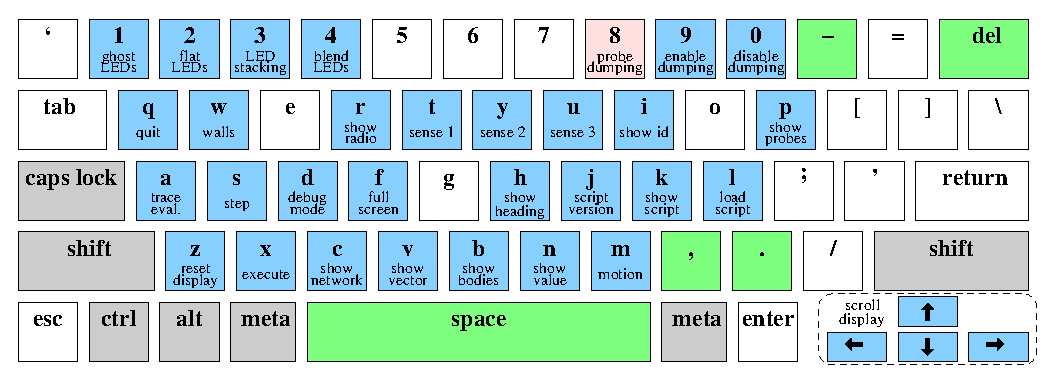
\includegraphics[width=6in]{figures/keyboard-lower.eps}
\caption{Lower case keyboard assignments}
\end{figure}

\begin{figure}[hp]
\centering
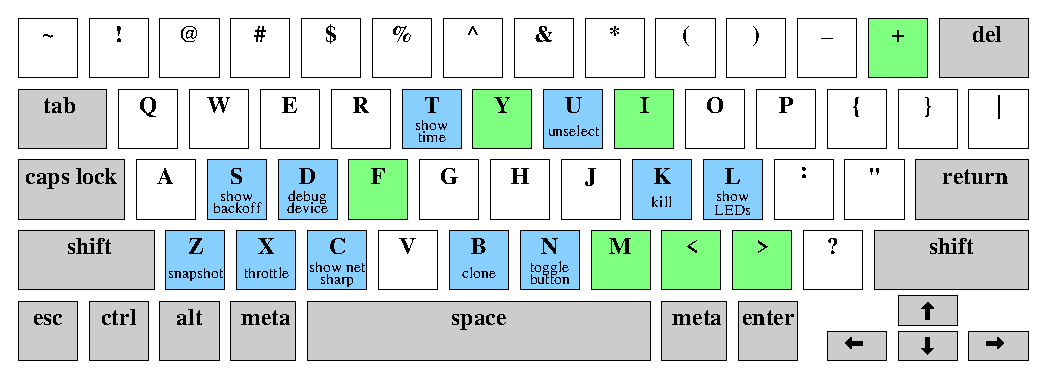
\includegraphics[width=6in]{figures/keyboard-upper.eps}
\caption{Upper case keyboard assignments}
\end{figure}

\begin{figure}[hp]
\centering
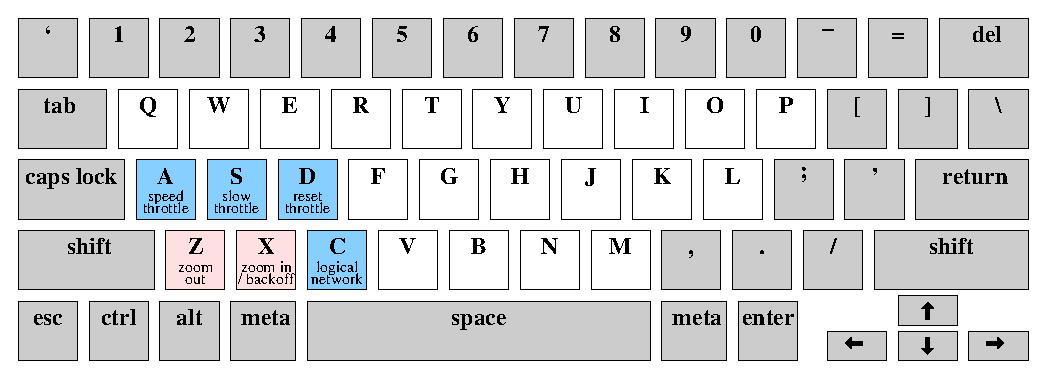
\includegraphics[width=6in]{figures/keyboard-ctrl.eps}
\caption{Control-key keyboard assignments}
\end{figure}

\section{Mouse Assignments:}

\begin{center}
\begin{tabular}{|l|cccc|}
\hline
BUTTON & CLICK & DRAG & SHIFT-CLICK & SHIFT-DRAG \\ \hline
LEFT   & select & rotate & --- & select region \\
RIGHT  & print & zoom & --- & move devices \\
MIDDLE & --- & --- & --- & --- \\
\hline
\end{tabular}
\end{center}

\end{appendix}

\end{document}
